\chapter{Experiments} 

For the designed system we haven chosen multiple experiments to
verify its accuracy. Experiments in this part focus on the localization process
and overall experiments. The tracker experiments are located in the chapter
\ref{ch:tracker}.

\section{Calibration and localization}
\label{s:experiment-static}

In order to measure a quality of calibration and localization we exclude a
tracking component. Therefore, we propose an experiment with static points in a
camera views. Then we estimate a position in 3D for these points.

It is complicated to measure distance from the origin of the coordinate system,
i.e. point inside the first camera to any given point. Therefore, we measure
distances between the static points in the real world and compute the distance
between their estimated position in 3D coordinates. Then we compare the results.

To skip the tracking part, we created a new tracker.  The new tracker always
returns the same position.  Doing this, we excluded tracker from our process.

We have chosen the grid as in the Figure \ref{fig:grid} as our pattern for experiments.
The vertical lines are circa 400~mm long and the distance between them is circa
200~mm. We measured distances between the crossings. We numbered the crossing,
the left column is from top to the bottom from 1 to 7 and the right column from
8 to 14 (see the Figure \ref{fig:ladder_numbered}).

The setup of the cameras was nearly parallel, which means, the center rays of
their views were parallel, looking in same direction. The distance between them
was circa 16~cm. Selected points are displayed in the Figure
\ref{fig:ladder_ground}. 

We repeated the experiment ten times, with exactly same setup in order to get
more reliable results. The only difference was the frames chosen for the
calibration (frames for the calibration were randomly chosen from the same
video). The number of the frames was same in each run. Therefore, we obtained
slightly different calibration data on the same setup.

With each set of calibration data we estimated position of the static points.
Then we computed distances between them. From such results from ten runs, we
computed average errors.

The results are listed in the table \ref{table:distances}. First two columns
define the pair of point between which are the results in corresponding row.
Third column denote the real length. The first column of the rests display the
average absolute error. Next columns display its relative value. The last
column displays the sample standard deviation for absolute error. 

To observe the results better, we have used also box plot displayed in the
Figure \ref{fig:horizontal-boxplot}. This box plot represents same results from the
same experiment. The orange line for each pair of points represent median of
the results. The 50\% of the results lies within the box. We denote height of
the this box as interquartile range (IQR). The whiskers represents all other
measurements, which lies at most one and half of the IQR away from the box. All
measurement which do not belong in previously mentioned groups are considered
as outliers and  will be displayed as circles.

\begin{figure}
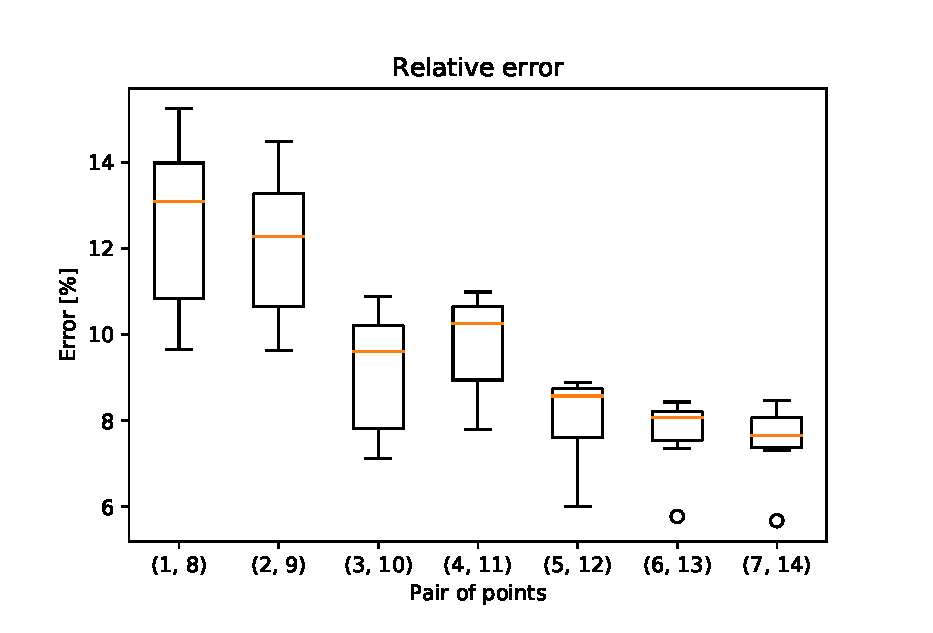
\includegraphics[width=\linewidth]{experiments/horizontal.eps}
\caption{Box plot of relative errors of estimated horizontal distances between the columns}
\label{fig:horizontal-boxplot}
\end{figure}

Based on the results displayed in the table \ref{table:distances} and the box
plot \ref{fig:horizontal-boxplot} we can see that estimated results are least accurate
for the points furthest from the cameras. Movement by few pixels so far away
from the camera means great real movement.  On the other hand, the
movement by same amount pixels closer to the camera means far smaller
real distance. Because of that, the error is expected to increase for
further points.

On the contrary, we can see that results too close to the camera are actually a
bit less accurate than the results close to the center of the view. The points
close to the camera are at the edge of the view. These less accurate results
may be caused by wrongly estimated distortion coefficients, as distortion
coefficients have major effect at the edges of the image.

Other box plots for the same setup with displayed results for the left and
right column, and for the perpendicular plane are displayed in the Appendix
\ref{ss:16results}.

\begin{table}
\centering
\begin{tabular}{|r|r|r|r|r|r|}
\hline
\multicolumn{2}{|c|}{Points} & \multicolumn{1}{c|}{Real} & \multicolumn{3}{c|}{Error} \\ 
\cline{1-2} \cline{4-6}
From & To & length [mm] & Average [mm] & Average [\%] & Std. dev. [mm]\\
\hline
\hline
\input{distances.txt}
\hline
\end{tabular}
\caption{Results of the experiment focused on the distances}
\label{table:distances}
\end{table}

We were interested if the results are good not only on the one plane -- in our
case the ground -- but also in the others. Now we have tested the precision in
two axes, which were perpendicular to each other (vertical and horizontal
lines). We have noticed, that the results for the vertical lines are less
precise. Therefore, we decided to test the last axis and its precision. We place
a wall with the marks, which is perpendicular to the ground and measured the
distance between the marks. The setup can be seen in the Figure
\ref{fig:table}. The marks are numbered as displayed in the image
\ref{fig:tablenumbered}. The results are included in the table
\ref{table:distances}. 

We did the same experiment with another setup, when the cameras were 63~cm
apart from each other. We were interested, if the results are better in
parallel setup, or not. Based on the results, the parralel setup performed
better when the lines were parrlalel to the camera X-axis (i.e. horizontal). On
the other hand, the setup with cameras far from each other and not having
parralel view performed better in measuring non-horizontal lines. 

\todo[inline]{A preco?}

The results for this second experiment are listed in the appendix in the
section \ref{ss:63results}. Same numbering of the marks was used.

\begin{figure}
\centering
\includegraphics[width=0.8\linewidth]{img/experiments/right-ladder-numbered.png}
\caption{Numbering the points}
\label{fig:ladder_numbered}
\end{figure}

\begin{figure}
\centering
\begin{subfigure}{0.48\linewidth}
	\includegraphics[width=\linewidth]{img/experiments/left-ladder.png}
\end{subfigure}
\begin{subfigure}{0.48\linewidth}
	\includegraphics[width=\linewidth]{img/experiments/right-ladder.png}
\end{subfigure}
\caption{Selecting the points from the videos}
\label{fig:ladder_ground}
\end{figure}



\begin{figure}
\centering
\begin{subfigure}{0.48\linewidth}
	\includegraphics[width=\linewidth]{img/experiments/table-left.jpg}
	\caption{Left view of the camera with marks}
	\label{fig:tablenumbered}
\end{subfigure}
\begin{subfigure}{0.48\linewidth}
	\includegraphics[width=\linewidth]{img/experiments/table-right.jpg}
	\caption{Right view of the camera}
\end{subfigure}
\caption{The views of the camera on the perpendicular plane to the ground}
\label{fig:table}
\end{figure}

\begin{figure}
\centering
\begin{tikzpicture}[]
	\draw (0, 0) -- (12, 0);
	\draw (0, 4) -- (12, 4);	
	\draw (0, 0) -- (0, 4);
	\draw (2, 0) -- (2, 4);
	\draw (4, 0) -- (4, 4);
	\draw (6, 0) -- (6, 4);
	\draw (8, 0) -- (8, 4);
	\draw (10, 0) -- (10, 4);
	\draw (12, 0) -- (12, 4);
	\node [right] at (0.1, -0.25) {200mm};
	\node [right] at (2.1, -0.25) {200mm};
	\node [right] at (4.1, -0.25) {200mm};
	\node [right] at (6.1, -0.25) {200mm};
	\node [right] at (8.1, -0.25) {200mm};
	\node [right] at (10.1, -0.25) {200mm};
	\node [right] at (12.1, 2) {400mm};
\end{tikzpicture}
\caption{Pattern used for experiments}
\label{fig:grid}
\end{figure}

\section{Complex experiments}

As the last step, we decided to test the whole system in a real environment. This
time we included all parts of the application -- calibration, tracking and also
localization. In the previous experiments, we tested the liability of the
trackers and the precision of the results. Now we test the usability of the
system as the whole.

\subsection{Experiment with the one small object}

The most important experiment -- the experiment which decides if the system is
usable -- is experiment under real conditions. We created a square to follow by
autonomous robot. This square have the length of the side equal 14.5~cm (see
Figure \ref{fig:robot-square}). The robot did four laps around the square. It
speed was circa \todo[inline]{Aky rychly robot}. For tracking we used \hsv{}
tracker. The results are displayed in the Figure \ref{fig:square-results}.

We can see in the left picture, that the drawn line is similar to our shape.
Not having sharp edges, since our robot turns in the bends over the inner
wheel. On the other hand, the results from the another view are not so amazing.
The coordinates have a lot of noise over Z-axis. This noise is under 5~cm, on
average 1.4~cm. The noise is only present, if the robot is following horizontal
lines of the square. This corresponds to our theory mentioned in the Section
\ref{s:}, since the camera views are not parralel, so the horizontal lines are
less precise.
\todo[inline]{Odkaz na section}

As the last step we computed maximum of the distances between any two points,
which were located. In this case, the expected value the length of the
diagonal, which is equal to 20.5061~cm. Our results are between 18.54~cm to
19.38~cm, depending on the run. That means, that the error is only usually
between 1 and 2~cm. This corresponds to previously measured inaccuracy in
non-parralel alignment.

\begin{figure}
\includegraphics[width=\linewidth]{img/experiments/square-robot.png}
\caption{Experiment with the robot}
\label{fig:robot-square}
\end{figure}

\begin{figure}
\centering
\begin{subfigure}{0.48\linewidth}
	\includegraphics[width=\linewidth]{img/experiments/square-nice.png}
\end{subfigure}
\begin{subfigure}{0.48\linewidth}
	\includegraphics[width=\linewidth]{img/experiments/square-ugly.png}
\end{subfigure}
\caption{Results of the localization -- four laps by the robot}
\label{fig:square-results}
\end{figure}

\subsection{Experiment with two objects}

This experiment will test the ability of the system to track multiple objects.
This effectively exclude \simback{} tracker as it is not able to track multiple
objects. Furthermore, we track objects with multicolored surface, making \hsv
tracker also unusable. The rest of the trackers are mostly slower, more
problematic.

We can see the setup for the experiment in the Figure \ref{fig:two-init}. We
can see two boxes, both in shades of blue. During testing many trackers failed
to track the object and lost it. We chose the \corr{} tracker as it provided
best results. It is medium fast tracker. The tracker sometimes lost the
images, but most of the time it was able to track. Because of the object lost,
sometimes an interaction of the user is needed, to reinitialize a tracker.

Sample results of the trajectories for two objects are displayed in the Figure
\ref{fig:two-trajectories}. During the experiment, the boxes were moving
between the yellow marks and swapped places. We can see these four marks easily
as the points, where the trajectories significantly changed directions. 

\begin{figure}[p]
\includegraphics[width=\linewidth]{img/experiments/two-objects.png}
\caption{Initialization of the two objects}
\label{fig:two-init}
\end{figure}

\begin{figure}
\centering
\begin{subfigure}{0.48\linewidth}
	\includegraphics[width=\linewidth]{img/experiments/trajectories1.png}
\end{subfigure}
\begin{subfigure}{0.48\linewidth}
	\includegraphics[width=\linewidth]{img/experiments/trajectories2.png}
\end{subfigure}
\caption{Sample trajectories from tracking two objects}
\label{fig:two-trajectories}
\end{figure}
